% This LaTeX was auto-generated from MATLAB code.
% To make changes, update the MATLAB code and republish this document.

\documentclass{article}
\usepackage{graphicx}
\usepackage{color}

\sloppy
\definecolor{lightgray}{gray}{0.5}
\setlength{\parindent}{0pt}

\begin{document}

    
    
\subsection*{Contents}

\begin{itemize}
\setlength{\itemsep}{-1ex}
   \item Get utility functions
   \item Open data
   \item Visualisation
   \item Test for integrating effects
   \item ARIMA model for CO2
   \item CO2 Change points
\end{itemize}
\begin{verbatim}
clear; close all;
\end{verbatim}


\subsection*{Get utility functions}

\begin{verbatim}
[f1,f2] = utils();
\end{verbatim}


\subsection*{Open data}

\begin{verbatim}
path = "./Data/india_data.xlsx";
% opts = detectImportOptions(path);
T = readtable(path,"ReadRowNames",true);
data = table2array(T)';
% Finding the first NAN value and taking data upto the instance before it
cut_off = length(data(:,1));
for i = 1:length(data(:,1))
    if (sum(isnan(data(i,:))))
        cut_off = i-1;
        break;
    end
end
time = data(1:cut_off,1);
Data = data(1:cut_off,2:end);
\end{verbatim}


\subsection*{Visualisation}

\begin{verbatim}
n = length(time);
m = length(Data(1,:));
subplot(2,1,1);
plot(time,Data(:,1));
title('CO2 emissions');
ylabel('CO2 emissions in idk'); xlabel('Year');
subplot(2,1,2);
plot(time,Data(:,2));
title('GDP');
ylabel('GDP in idk'); xlabel('Year');
% From the plot we see non-stationarity of trend type (not random walk) as
% would be expected.
\end{verbatim}

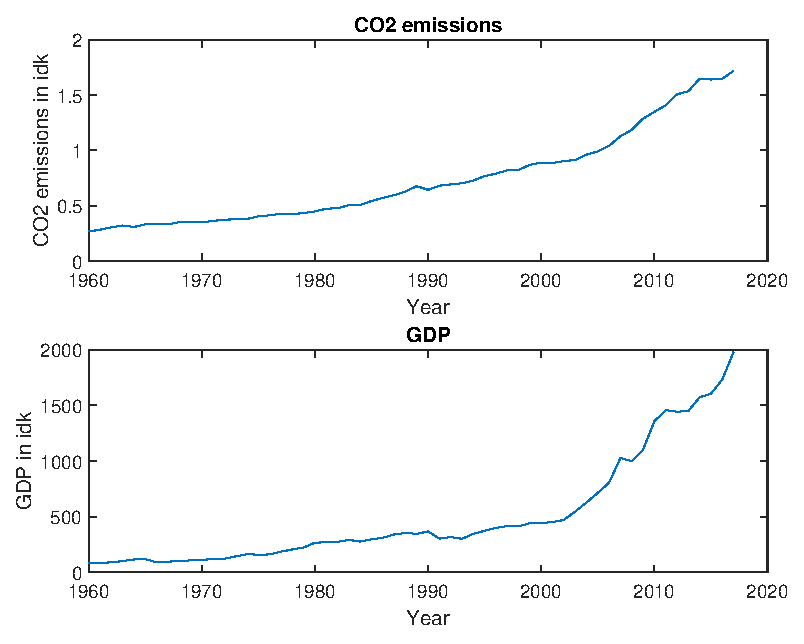
\includegraphics [width=4in]{univariate_analysis_01.eps}


\subsection*{Test for integrating effects}

\begin{verbatim}
results = zeros(m,2);
for i = 1:m
    [results(i,1), results(i,2)] = adftest((Data(:,i)));
end
% Unit root hypothesis not rejected for both GDP and CO2 => has integrating
% effects
CO2 = (Data(:,1));
diff_CO2 = diff(CO2);
[hCO2,pCO2] = adftest(diff_CO2);
diff_GDP = diff(Data(:,2));
[hGDP,pGDP] = adftest(diff_GDP);
figure;
subplot(211);plot(time(2:end),diff_CO2);title("Differenced CO2");xlabel("Time");
subplot(212);plot(time(2:end),diff_GDP);title("Differenced GDP");xlabel("Time");
% Null hypothesis rejected, the differenced series does not have any
% integrating effects!
\end{verbatim}

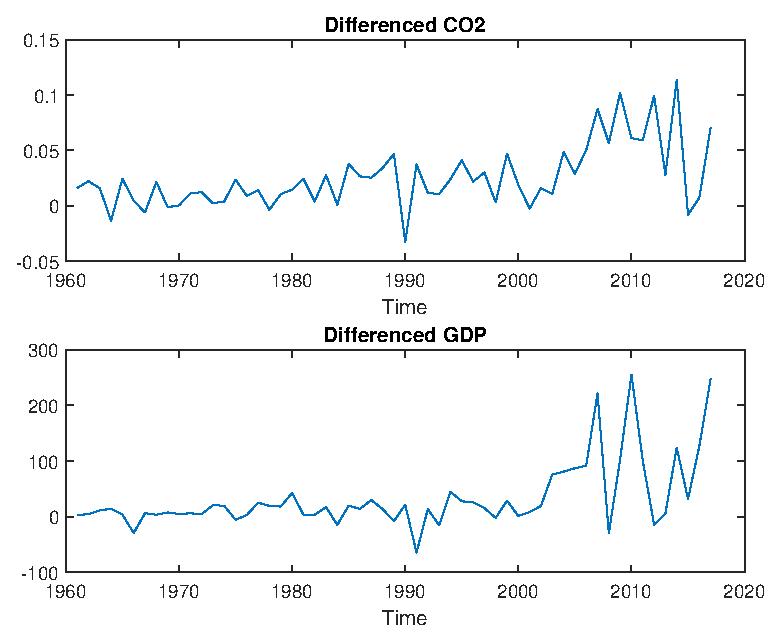
\includegraphics [width=4in]{univariate_analysis_02.eps}


\subsection*{ARIMA model for CO2}

\begin{verbatim}
figure;
subplot(211); autocorr(diff_CO2); title('ACF diff_CO2');
subplot(212); parcorr(diff_CO2,"NumLags",30); title('PACF diff_CO2');
[est_m1,res,uf,of] = f1([1,1,1],1,CO2,0,0);
% Residuals are white! so no underfitting. All coefficients except constant
% term are significant
[est_m2,res2,uf2,of2] = f1([1,1,1],0,CO2,0,0);
% Neither underfit nor overfit!
\end{verbatim}

        \color{lightgray} \begin{verbatim} 
    ARIMA(1,1,1) Model (Gaussian Distribution):
 
                  Value       StandardError    TStatistic      PValue  
                __________    _____________    __________    __________

    Constant     0.0012076      0.0018292       0.66015         0.50915
    AR{1}          0.98093       0.062976        15.576       1.057e-54
    MA{1}         -0.83351        0.13358       -6.2396      4.3879e-10
    Variance    0.00059875      8.779e-05        6.8202      9.0912e-12

Warning: Upper bound constraints are active; standard errors may be inaccurate. 
 
    ARIMA(1,1,1) Model (Gaussian Distribution):
 
                  Value       StandardError    TStatistic      PValue   
                __________    _____________    __________    ___________

    Constant             0              0           NaN              NaN
    AR{1}                1       0.031197        32.054      1.9014e-225
    MA{1}         -0.80292        0.10952       -7.3311       2.2829e-13
    Variance    0.00061695     9.0215e-05        6.8386       7.9943e-12

\end{verbatim} \color{black}
    
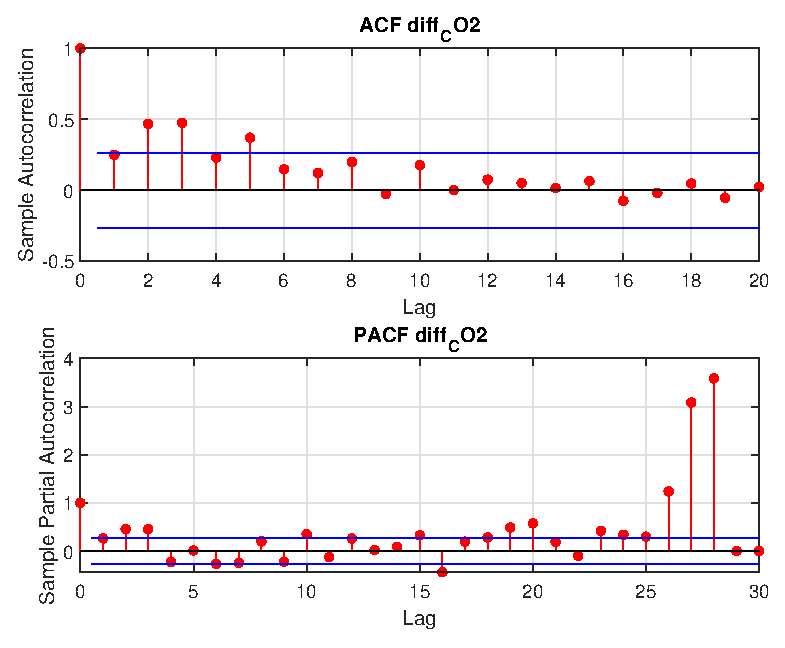
\includegraphics [width=4in]{univariate_analysis_03.eps}


\subsection*{CO2 Change points}

\begin{par}
We find approximately where the mean changes using findchangepts and also observe visually to detect variance/mean changes
\end{par} \vspace{1em}
\begin{verbatim}
figure;findchangepts(res2,'MaxNumChanges',3);
ipt = findchangepts(res2,'MaxNumChanges',3);
fspec = 'Variance before the first change point = %f \n Variance in the second region %f';
fprintf(fspec,var(res2(1:ipt(1))),var(res2(ipt(1):ipt(2))));
% third region variance ignored because the region is too small
all_pts = [ipt; 31];
% 31 included because it has a huge dip
% Noting down the years
cpts_year = time(all_pts);
\end{verbatim}

        \color{lightgray} \begin{verbatim}Variance before the first change point = 0.000292 
 Variance in the second region 0.001647\end{verbatim} \color{black}
    
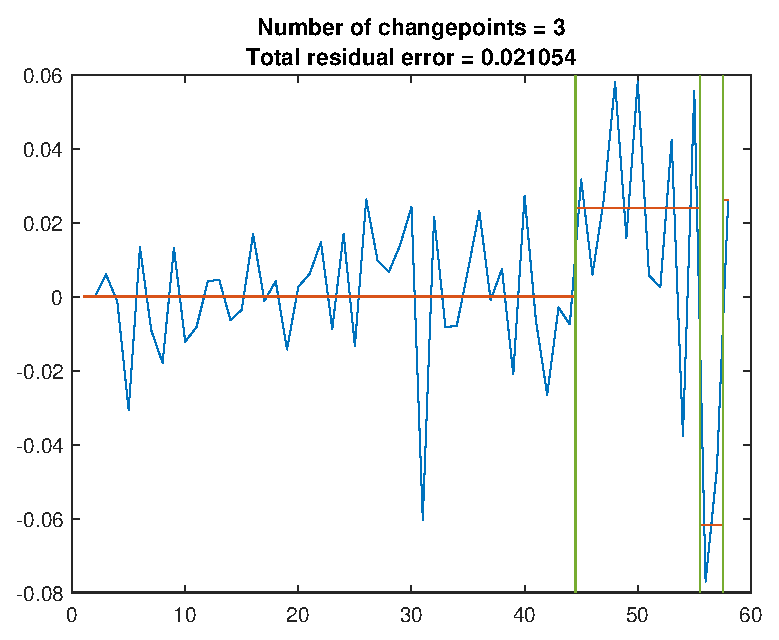
\includegraphics [width=4in]{univariate_analysis_04.eps}



\end{document}

